\documentclass[border=0mm]{standalone}
\usepackage{pgfplots}
\usepgfplotslibrary{groupplots}
\pgfplotsset{compat=1.17}
\usepackage{xcolor}
\usepackage{xstring}
\usepackage{tikz}
\usepackage{eqparbox}


\definecolor{color1}{rgb}{0,0.4470,0.7410}
\definecolor{color2}{rgb}{0.8500,0.3250,0.0980}
\definecolor{color3}{rgb}{0.9290,0.6940,0.1250}
\definecolor{color4}{rgb}{0.4940,0.1840,0.5560}
\definecolor{color5}{rgb}{0.4660,0.6740,0.1880}
\definecolor{color6}{rgb}{0.3010,0.7450,0.9330}


\begin{document}

\pgfplotsset{
compat=1.11,
legend image code/.code={
\draw[mark repeat=2,mark phase=2]
plot coordinates {
(0cm,0cm)
(0.3cm,0cm)        %% default is (0.3cm,0cm)
(0.6cm,0cm)         %% default is (0.6cm,0cm)
};%
}
}%

\pgfdeclarelayer{background layer}%
\pgfdeclarelayer{foreground layer}%
\pgfsetlayers{background layer,main,foreground layer}%

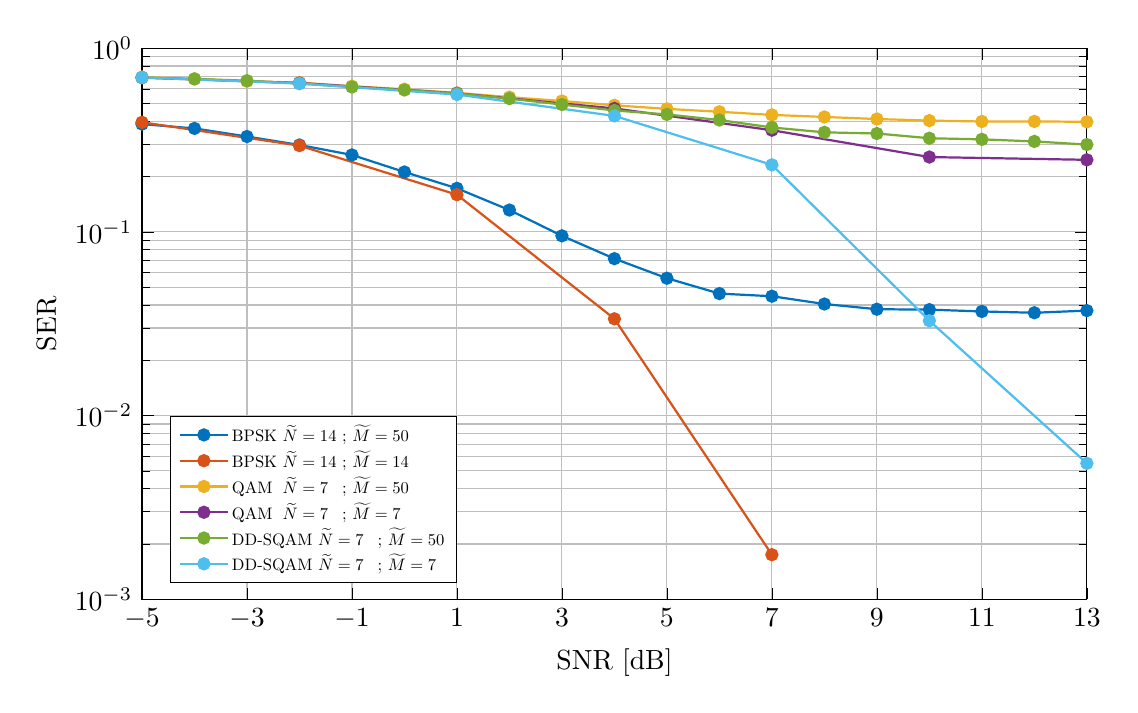
\begin{tikzpicture}[
]
\begin{semilogyaxis}[%
width=12cm,
height=7cm,
scale only axis,
every outer x axis line/.append style={black},
every x tick label/.append style={font=\color{black}},
every x tick/.append style={black},
xmin=-5,
xmax=13,
xlabel={SNR [dB]},
every outer y axis line/.append style={black},
every y tick label/.append style={font=\color{black}},
every y tick/.append style={black},
ymin=0.001,
ymax=1,
ylabel={SER},
axis background/.style={fill=white},
xmajorgrids,
ymajorgrids,
yminorgrids,
xtick={-5,-3,...,13},
legend pos=south west,
legend style={nodes={scale=0.6, transform shape}},
legend cell align={left},
]

\addplot [thick,color1, mark=*] coordinates {(-5,0.3861500024795532)(-4,0.3658500015735626)(-3,0.33044999837875366)(-2,0.29725000262260437)(-1,0.2623499929904938)(0,0.21185000240802765)(1,0.17264999449253082)(2,0.1315000057220459)(3,0.09520000219345093)(4,0.07150000333786011)(5,0.05595000088214874)(6,0.046149998903274536)(7,0.04464999958872795)(8,0.04050000011920929)(9,0.037950001657009125)(10,0.0377499982714653)(11,0.03689999878406525)(12,0.03629999980330467)(13,0.037300001829862595)};
\addlegendentry{\eqmakebox[m1][l]{BPSK} $\widetilde{N}=14$ ; $\widetilde{M}=50$}

\addplot [thick,color2, mark=*] coordinates {(-5,0.3950999975204468)(-2,0.2948000133037567)(1,0.15940000116825104)(4,0.033649999648332596)(7,0.0017500000540167093)(10,0.0)(13,0.0)};
\addlegendentry{\eqmakebox[m1][l]{BPSK} $\widetilde{N}=14$ ; $\widetilde{M}=14$}


\addplot [thick,color3, mark=*] coordinates {(-5,0.6963000297546387)(-4,0.6811000108718872)(-3,0.6604499816894531)(-2,0.6498000025749207)(-1,0.6211000084877014)(0,0.5978500247001648)(1,0.5709999799728394)(2,0.5414999723434448)(3,0.5156999826431274)(4,0.48855000734329224)(5,0.4672999978065491)(6,0.4505999982357025)(7,0.4332500100135803)(8,0.42225000262260437)(9,0.4115000069141388)(10,0.40334999561309814)(11,0.3989500105381012)(12,0.3993000090122223)(13,0.39739999175071716)};
\addlegendentry{\eqmakebox[m1][l]{QAM} $\widetilde{N}=7\phantom{0}$ ; $\widetilde{M}=50$}

\addplot [thick,color4, mark=*] coordinates {(-5,0.6909000277519226)(-2,0.6460999846458435)(1,0.567799985408783)(4,0.4699000120162964)(7,0.357699990272522)(10,0.2554500102996826)(13,0.24674999713897705)};
\addlegendentry{\eqmakebox[m1][l]{QAM} $\widetilde{N}=7\phantom{0}$ ; $\widetilde{M}=7$}


\addplot [thick,color5, mark=*] coordinates {(-5,0.6919500231742859)(-4,0.6798999905586243)(-3,0.6654999852180481)(-2,0.6413999795913696)(-1,0.6147000193595886)(0,0.5920500159263611)(1,0.5661500096321106)(2,0.5313000082969666)(3,0.4934000074863434)(4,0.458050012588501)(5,0.4359000027179718)(6,0.40619999170303345)(7,0.3702000081539154)(8,0.34825000166893005)(9,0.34314998984336853)(10,0.32339999079704285)(11,0.31894999742507935)(12,0.31075000762939453)(13,0.2987000048160553)};
\addlegendentry{\eqmakebox[m1][l]{DD-SQAM} $\widetilde{N}=7\phantom{0}$ ; $\widetilde{M}=50$}

\addplot [thick,color6, mark=*] coordinates {(-5,0.693149983882904)(-2,0.642300009727478)(1,0.5590500235557556)(4,0.42800000309944153)(7,0.2316499948501587)(10,0.0328500010073185)(13,0.005499999970197678)};
\addlegendentry{\eqmakebox[m1][l]{DD-SQAM} $\widetilde{N}=7\phantom{0}$ ; $\widetilde{M}=7$}



\end{semilogyaxis}

\end{tikzpicture}


\end{document}
























